\documentclass{../exhibit}

\title{A $\pi$-rates EYE}

%% Font
\usepackage{imfellEnglish}
\usepackage[T1]{fontenc}
\raggedright

\usepackage{background}

\backgroundsetup{
scale=1,
color=black,
opacity=0.4,
angle=0,
contents={%
  \includegraphics[height=\paperheight]{mapBackground.jpg}%%https://upload.wikimedia.org/wikipedia/commons/8/81/Nautical_chart_of_the_West_Indies_1797.jpg
  }%
}




%% For the context
%% https://tex.stackexchange.com/questions/86150/torn-page-effect/86151#86151
\usepackage{tikz}
\usetikzlibrary{decorations.pathmorphing}
\definecolor{paper}{RGB}{239,227,157}





\renewcommand{\maketitle}{ %
  \begin{center}
    \scalebox{8}{\thetitle}
  \end{center}
  
\begin{tabular*}{\textwidth}{c @{\extracolsep{\fill}} c}  
\resizebox{4in}{!}{\begin{minipage}[b]{3in}\huge\directions\end{minipage}} &
  \resizebox{4in}{!}{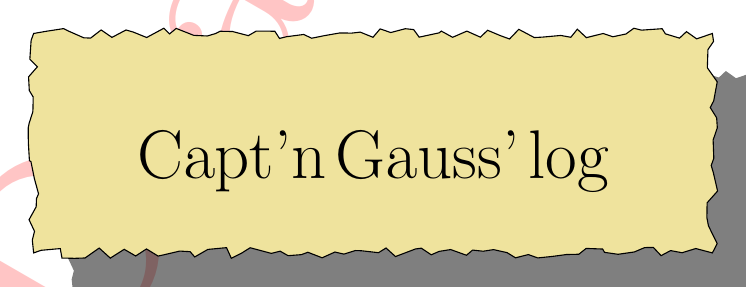
\begin{tikzpicture}[pencildraw/.style={ %
    decorate,
    decoration={random steps,segment length=4pt,amplitude=2pt}
    } %
]
\node[
preaction={fill=black,opacity=.5,transform canvas={xshift=.5cm,yshift=-.5cm}},
pencildraw,draw,fill=paper,text width=3in,inner sep=.5cm] 
{\begin{center}\Huge Capt'n Gauss' log \end{center}\vspace{.7cm} {\huge\context}};
\end{tikzpicture}}

\end{tabular*}

\vfill

\includegraphics[width=3in]{logoPirate.png}\hfill \includegraphics[width=2in]{bammLogo.png}


}


\begin{document}



\begin{context}
  
SHARP be the $\pi$-rates eye!


  \vspace{1cm}

Knowing numbers with just a glance, 

  \vspace{1cm}

a $\pi$-rates skill, useful still!

  
\end{context}



\begin{directions}
  Look at the cards:
  \begin{itemize}
  \item Count marks on the cards as fast as you can. \\ USE PATTERNS to help!
  \item How many can you get \\before time runs out?
  \end{itemize}
\end{directions}



\begin{example}
  \begin{center}
    \begin{tabular}{lr}
      \raisebox{-2in}{\includegraphics[width=.4\textwidth]{dots.png}} &
      \quad\quad\begin{minipage}{.4\textwidth}
        Here we see\\[1cm]
        FIVE groups of TWO\\[1cm]
        so there are TEN!
      \end{minipage}
    \end{tabular}
  \end{center}
\end{example}




\begin{mathConnections}
  https://bartsnapp.github.io/Math-Outreach-Exhibits/subitizing/
\end{mathConnections}
\end{document}
